\documentclass[11pt, twocolumn]{article}

\usepackage[english]{babel}
\usepackage[utf8x]{inputenc}
\usepackage[T1]{fontenc}

%\usepackage[nottoc,numbib]{tocbibind} % References section appears in toc
\usepackage[colorlinks=true, allcolors=blue]{hyperref}
\usepackage{graphicx}

\title{Bypassing DRM protections and countermeasures}
\date{\today}
\author{Bastien DHIVER \\ \href{mailto:bfrd2@kent.ac.uk}{bfrd2@kent.ac.uk}}

\begin{document}
\maketitle

%\tableofcontents
%\clearpage

\begin{abstract}
	This monograph will provide to the reader an overall view on the Digital Rights Management (DRM) protections as well as the most common ways used to bypass them along with some techniques to harden their analysis.
\end{abstract}

\section{Introduction}

"[in the media industry] DRM is used by content distributors to restrict the way in which content may be used, transferred, and stored by users." \cite{Wang:2013}

DRM protections have been around for quite some time now as well as an ongoing arms race between their designers and those who circumvent them.
The protections are often bypassed for financial aspects.
Users are not often willing to pay for content that is also available for free on the Internet.
Protecting media content is not a trivial task as we will see, especially when the content is stored on the user's computer.
Bypassing techniques are numerous and some of them require almost no technical skills.
The defensive side uses anti-bypass techniques that are closely related in some extent to protections used by malwares.

\section{DRM Protections}

DRM technologies are highly complex and extensive~\cite{Michiels:2005}.
They must be designed in a way that is it very hard for a consumer to access the content either by retrieving the decryption key or dumping the decrypted content.
This is not a trivial task at all since DRM clients are executed on end user's devices which are potentially fully controlled by them.
The figure \ref{fig:drm} gives an overview \footnote{https://www.usenix.org/sites/default/files/conference/protected-files/wang1\_sec13\_slides.pdf} of the steps taken by a DRM system in a video streaming service, .

\begin{figure}[ht]
	\centering
	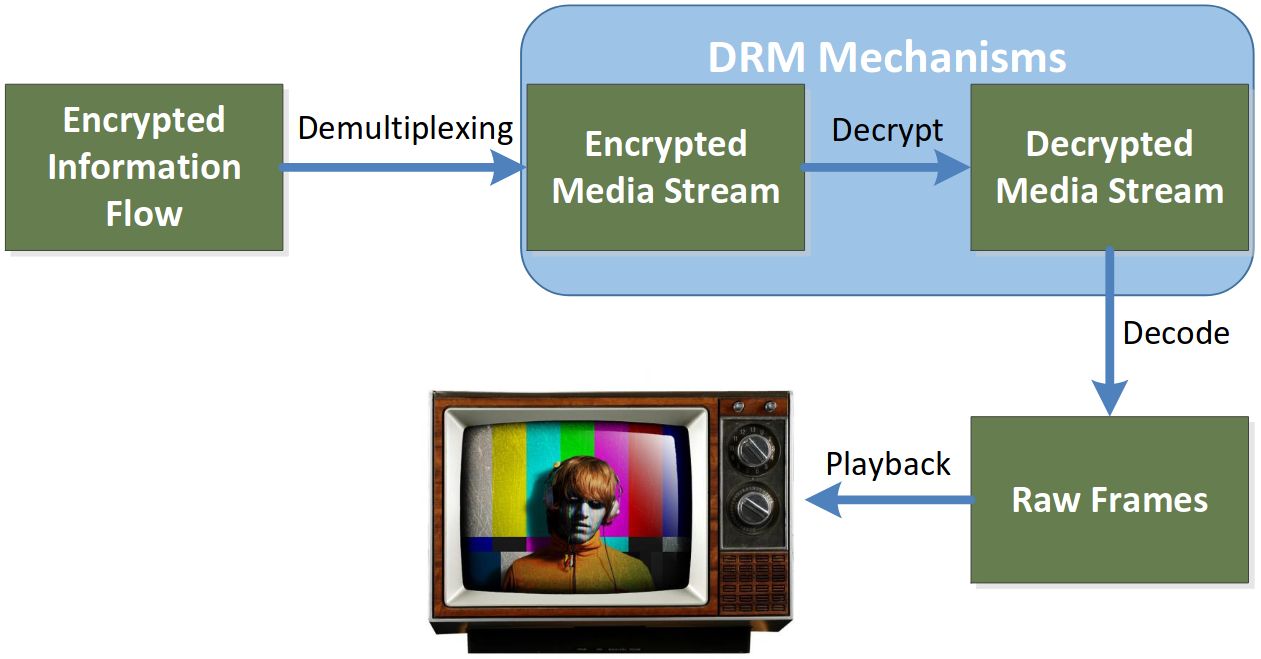
\includegraphics[scale=0.18]{images/HowDRMWorks.png}
	\caption{How DRM works}
	\label{fig:drm}
\end{figure}

DRM help to retain some control on the distributed digital content but only after it had been delivered.
Such enforced restrictions can be to prevent a copy to be made, to limit the number of reads/plays (also across devices), set up time limits, reduce the forwarding abilities or ensure that only authorized users are accessing the content.
Two main classes of DRM schemes exists, the ones that are using encryption and the ones that aren't.

A myriad of DRM schemes exists.
Here is a short non-exhaustive list: XCP, MediaMax, DVD CSS, WMDRM, FairPlay, Adobe PDF Merchant/WebBuy, Microsoft PlayReady, RTMPE and Spotify's content protection.
Few of them are described and analysed over the literature~\cite{Wang:2013}\cite{Michiels:2005}\cite{Halderman:2006}.
It is worth pointing out that the vast majority are proprietary technologies.
Security by obscurity, designs kept secret and an over-reliance on cryptography are properties of such systems.
Open standards exist such as the MPEG-21 framework, Coral, Marlin and the Open Mobile Alliance framework.
The latter is is an open-standards based framework that has been widely adopted as the de facto standard in the mobile industry.

"DRM technologies must support a diversity of devices, users, platforms, and media, and a wide varitety of system requirements concerning security, flexibility, and manageability."\cite{Michiels:2005}
In order to achieve this support, decryption process is sometimes moved outside of the computer because of trust issues with client's devices.
Hardware-based DRM have been created for this purpose and can for example be used to protect a software by requiring a physical dongle that is not duplicable to be provided.
Link-protection schemes closer to the hardware aim to protect content in transit.
Compliant hardware is required.
The High-bandwidth Digital Copy Protection (HDCP) schemes is one of those.
It can be used with connections such as DisplayPort, Digital Visual Interface (DVI) and HDMI for example.
Implementing such DRM hardware protections is difficult, costly and doesn't always meet usability criteria.
The upgrade process can be challenging for instance.

Three major challenges are at the heart of new DRM schemes according to \cite{Michiels:2005}. Namely, (1) the fragmentation of individual solutions, (2) the limited reuse and interoperability and (3) the software architecture support.

\section{Bypassing techniques}

Bypassing techniques have been around for quite some time \cite{Hauser:2003}.

The first bypassing technique that comes to mind is the analogue hole.
The analogue hole is when content is captured in an analogue form.
We can think of a user using a screen recorder software when watching a movie on his computer.
This flaw is due to the fact that the media must be consumed by a human.
However, humans cannot decrypt content on the fly with their brains (yet).
The downside of this technique is a loss of quality in the process because re-encoding the audio and video signals is mandatory.
DRM cannot prevent such attacks.
To not lose quality inherent to the analogue hole, the recording must take place just after decryption, before decoding, when the decrypted media stream is available as shown on Figure \ref{fig:drm}.
This recoding can be done with two ways, either recover the keys used to encrypt the content or intercept decrypted content.

Reverse engineering techniques are widely used to analyse DRM, find weaknesses and exploit them.
An early example is found with a popular cryptographic DRM used on DVD which is the Content Scramble System (CSS).
It has been broken in 1999 after that a group of researchers used reverse engineering techniques to identify the encryption algorithm used in DVD players.
The most famous tools used to reverse engineer programs are OllyDBG and IDA Pro.
A classical approach is to use a debugger, set breakpoints on file I/O and memory access and try to find the code that could lead to the decryption algorithm.
Sometimes a very little modification \cite{Choi:2016} such as removing a conditional jump instruction (two bytes) is sufficient to bypass a critical check as shown by figure \ref{fig:bypass}.
\begin{figure}[ht]
	\centering
	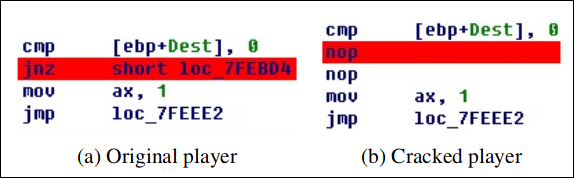
\includegraphics[scale=0.4]{images/asmBypass.png}
	\caption{Verification procedure is disabled by replacing the jnz instruction with nop instructions that do nothing \cite{Choi:2016}}
	\label{fig:bypass}
\end{figure}
Code coverage technique can help to find relevant code in large binaries, especially to identify code blocks that are used at runtime.
As we know that decryption must come at some point in the process, analysing the flow of data between buffers can also help to identify the transition between encrypted and decrypted data in a media player and can even be a semi-automated process \cite{Wang:2013}.
Key recovery have been proven to be possible as shown with the DeCSS case or the HDCP master keys compromision\footnote{https://rudd-o.com/monopolies-of-the-mind/the-hdcp-master-key}.
Since DRM protections are not just about a piece of software, their architecture, actors and relations between them can also be exploited.
They are mainly divided in four parts: the DRM agent, the Content Issuer (CI), the Rights Issuer (RI), and the user.
Bypassing either, the checks for permissions and constraints between the DRM agent and the Rights Issuer, or the integrity check of the right object can lead to be granted full access by the system.
One can also take advantage of the operating system components to capture data from the player to the driver or capture data when passing from the driver to the hardware by emulating an alternative audio card for example.
Dumping and analysing network traffic can sometimes help to discover activation process information\footnote{http://bit.ly/reconcx-2016-audible-drm}.

It is \textbf{impossible} to prevent reverse engineering on open system.
A secret can't really be hidden in a software.
But one can increase the difficulty of such a task.
We now have a sense of how difficult it is to securely implement a DRM agent in the real-world.

\section{Countermeasures}

The defensive side has at its disposal a plethora of counter techniques.

Since rootkits will (hopefully) no longer be used after the Sony-BMG's CD DRM case~\cite{Halderman:2006} debacle, approaches to hide critical codes and control flows when it comes to software are used in order to slow down as much as possible attackers.
This seems to be the only way to dissuade them.

Anti-reverse engineering techniques are used to do so \cite{Newger:2016}.
The static view of the code can be confused in multiple ways using encrypted or "packed" object code, false disassembly, self-modifying code, \dots.
A good specific reference for the Windows operating system is given by Symantec\footnote{https://www.symantec.com/connect/articles/windows-anti-debug-reference}.
Anti-debugging techniques are popular as well to confuse the dynamic view of the code.
They use checks to detect if a debugger is present, interact with threads that may confuse the debugger and code tricks for instance.
Hide program's implementation details and functionality via code obfuscation is widely used.
The code is made more difficult to understand.
It forces the attacker to analyse a larger amounts of code and waste time observing dead code.
This is the opposite of good software engineering: inject junk code, embbed virtual machines, occupy the debug registers and using them to alter control flow, check of critical APIs for breakpoints opcodes, heavy use of exceptions to interrupt flow on execution, dispatching code jumps via a central point in a non-standard way, P-Code machine which encapsulates the decryption and key setup algorithms are just the tip of the iceberg.
"Using mechanisms like Virtual Machines to carry out the core protection algorithms is a very good technique and will probably become more important in newer protection mechanisms"\cite{Newger:2016}.
Security by obscurity is the rule for client applications.

Alternative ways such as trusted computing relying on a chain of trust, secure soundcard drivers that ensure that no recording takes place, White-box cryptography\footnote{http://www.whiteboxcrypto.com/files/2012\_misc.pdf} are implemented though various forms.
Self integrity checks of the application's code before the execution or at runtime to makes patching more difficult seems interesting.
"Such an integrity checking system can be used together with some hardware mechanism such as a Trusted Platform Module (TPM) or ARM TrustZone. Those mechanisms provide a means to reliably report the integrity of software and/or platform configurations with protected key storage to build a strong platform integrity verification mechanism by securely protecting the hash of the normal program binary image through a hardware chip embedded in the motherboard." \cite{Choi:2016}.
Tamper-resistant hardware is advised by researchers~\cite{Stamp:2003}.

Traitor tracing via watermarking is also used and is considered as the only viable option to add an almost unbreakable security~\cite{Hauser:2003}.
It's a discreet protection technology that doesn't prevent privacy but permit enforcement of a damage control policy.
In our case, watermarking is the binding technology that irreversibly attaches the identifier used for traitor tracing to the content in a robust way.
A presentation was given by my friend Théo and I as part of this module\footnote{http://bit.ly/CO834-watermarking-traitor-tracing}.
"In DRM context, the watermark must be able to survive indirect attacks such as audio and video grabbing."\cite{Ku:2004}
Watermarking provides a proof of ownership.
The system must be design in a way that once the watermark has been embedded in the content, it cannot be removed.
Also, fake watermark cannot be inserted, public key cryptography is used to this effect.
Resistance to collusion attacks is a must for the system to be efficient~\cite{Doerr:2010}.
Depending on the technique used by the attacker to retrieve the content, watermarks can be left almost intact as little or no quality loss is expected.

\section{Conclusion}

The most viable options seem to be the usage of tamper-resistant hardware for application integrity check combined with watermarking techniques in case the content gets leaked.
This battle will not be over soon.
Both parties always have more creative ways to outsmart each other.

%% --- References

\bibliography{refs}
\bibliographystyle{unsrt}

\end{document}
